\chapter{Float Features}

Examples for floats were already shown in \cref{fig:censorbox,tab:main_font_examples}.
These are mainly handled by the packages:
\begin{description}
    \item[\ctanpackage{caption}]
        The base package providing customizations for the caption text, for example
        automatic ending periods, which can be toggled globally.
    \item[\ctanpackage{svg}]
        Including \abb{scalable_vector_graphics} files using \LaTeX{}, or in this
        case \hologo{LuaLaTeX}, is not very straightforward.
        In fact, it is anything but: \abb{scalable_vector_graphics} files cannot
        be included directly at all and intermediate steps are needed.

        Using the \ctanpackage{svg} package, the workflow is somewhat automated.
        Only the original \abb{scalable_vector_graphics} files are kept as the
        \abb{single_source_of_truth}, and the generation of the
        \abb{portable_document_format} and accompanying \verb|.pdf_tex| files
        are left to the package.
        It calls InkScape for converting the \abb{scalable_vector_graphics} to
        \abb{portable_document_format} (or another format of choice), and if the
        \abb{scalable_vector_graphics} contains text to be included as \LaTeX{},
        a sidecar \verb|.pdf_tex| file is generated (the default behavior).
        To call InkScape, two requirements have to be met:
        \begin{enumerate}
            \item elevation aka \texttt{--shell-escape} is required to write
                external files, and
            \item InkScape has to be on the \verb|$PATH|, that means installed and
                subsequently registered.
                This is automatically done for Linux.
                If it is not done automatically on Windows, navigate to
                \emph{Edit the system environment variables} and add the directory
                containing \texttt{inkscape.exe} to the variable.
        \end{enumerate}
        Once the files are generated, they can be treated as temporary junk and are
        always easily regenerated from the source \abb{scalable_vector_graphics}.

        After years of experimentation, this seems like the best workflow.
        The only laborious manual task left is placement of annotations onto the
        generated \abb{portable_document_format} files.
        This seems like the best deal: no text is left in the
        \abb{scalable_vector_graphics} files themselves.
        Placing and debugging text in \abb{scalable_vector_graphics} files using
        the InkScape \textrightarrow{} \verb|PDF+PDF_TEX| route is \emph{very, very}
        annoying.
        This is because while InkScape offers text alignment operations
        (left, center, right) that translate into the embedded \verb|PDF_TEX|,
        the font cannot be known a priori while working on the
        \abb{scalable_vector_graphics}.
        Neither font size (most importantly its height), nor any other font
        property can be assumed.
        This also makes functions like \emph{Resize page to drawing or selection}
        futile if text is part of the outer elements of a drawing.

        Wanting to change any text later on results in having to start InkScape
        instead of just doing it conveniently in the \LaTeX{} source.
        The alternative is to place macros (\verb|\newcommand*{}|) everywhere
        inside the original \abb{scalable_vector_graphics}, where content should
        later be placed.
        These macros serve as labels, but are ugly, annoying, and remove the
        usability of the plain, original \abb{scalable_vector_graphics} file
        (since we would first need to know what each macro stands for).

        Using the \ctanpackage{svg} package to generate plain, text\-/less
        \abb{portable_document_format} and only later adding any
        text or annotation in the \LaTeX{} source itself seems the best of both
        worlds.
        \textbf{It certainly allows both tools to do what they're good at, and no more}:
        draw free\-/flowing vectors graphics with InkScape, then add text in
        \LaTeX{} (which can be done in \verb|\foreach| loops as well).
        An example for annotations (with loops) is shown in \cref{fig:bitmap_tikz}.
        All other graphics that are neither bitmaps nor \idx{tikz} graphics are
        handled using the \ctanpackage{svg} approach.

        All of this is very convenient indeed, since we can now do everything in
        \LaTeX{} and \ctanpackage{tikz} and basically never have to revisit the base
        \abb{scalable_vector_graphics} file, unless the graphic itself changes.
        All the labels stay in the \LaTeX{} source and are therefore also manageable
        through \texttt{git}.
    \item[\ctanpackage{floatrow}]
        A notable feature is the capability for captions the same width as the
        float they are attached to.
        This tends to look much tighter and tidier, see
        \cref{fig:wide_caption,fig:tighter_caption} for a comparison.

        Other features are automatic centering of floats, automatic positioning
        of captions (tables on top, figures below, independent of where the
        \verb|\caption| command occurs in the source), multiple floats and
        captions on the side.
        Depending on the aspect ratio of the image, positioning the caption besides
        the figure can look (subjectively) pretty, see \cref{fig:sidecap}.
\end{description}

\begin{figure}\ContinuedFloat*% Floats can be "continued" across pages like this
    % Conventional figure-syntax
    \includesvg[width=0.4\textwidth]{compressor_impeller_isometric}%
    \caption{%
        Example for a regular caption,
        spanning the whole width since it is so long.
        This can quickly look strange, especially if the figure itself is narrow%
    }%
    \label{fig:wide_caption}%
\end{figure}

\begin{figure}\ContinuedFloat
    % Optional argument \FBwidth causes graphic to be its actual size and caption
    % to take up the remaining space. Otherwise, horizontal space is split 50/50,
    % which doesn't make much sense.
    \ffigbox[\FBwidth]{%
        \caption{
            Example for a new caption, spanning just the width of the float
            it is attached to, despite the caption being much longer than the
            float is wide%
        }%
        \label{fig:tighter_caption}%
    }{%
        \includesvg[width=0.4\textwidth]{compressor_impeller_isometric}%
    }%
\end{figure}

\subsubsection{Multiple floats}

Other possibilities are rather arbitrary arrangements of sub\-/figures and -captions.
For this, see \cref{fig:multiple_floats}, which contains the two sub\-/figures
\cref{fig:multiple_floats_one,fig:multiple_floats_two}.
Multiple sub\-/tables are also possible, see \cref{tab:multiple_tables} with its four
sub\-/tables
\cref{tab:multiple_tables_one,tab:multiple_tables_two,tab:multiple_tables_three,tab:multiple_tables_four}.

\begin{figure}
    \ffigbox[\FBwidth]{%
        \begin{subfloatrow}[2]% Default is 2
            \ffigbox[\FBwidth]{%
                \includesvg[width=0.4\textwidth]{rotor_tip_clearance}
            }{%
                \caption{An example}%
                \label{fig:multiple_floats_one}%
            }%
            \ffigbox[\FBwidth]{%
                \includesvg[width=0.4\textwidth]{gas_volume}
            }{%
                \caption{Another example}%
                \label{fig:multiple_floats_two}%
            }%
        \end{subfloatrow}
    }{%
        \caption{%
            An example for sub\-/figures%
        }%
        \label{fig:multiple_floats}%
        \floatfoot{%
            This field can be used for a reference to a source:
            \adaptedfrom{} wherever%
        }%
    }%
\end{figure}

\begin{table}
    \small
    \floatbox{table}{
        %https://tex.stackexchange.com/q/295567/120853
        \begin{subfloatrow}
            \ttabbox[\FBwidth]{%
                \begin{tabular}{
                    @{}
                    m{0.25\textwidth}
                    m{0.15\textwidth}
                    @{}
                }
                    \toprule
                        Column One & Column Two\\
                    \midrule
                        Just & a \\
                        normal & table\\
                        Nothing & special.\\
                    \bottomrule
                \end{tabular}
            }{%
                \caption{Table One}%
                \label{tab:multiple_tables_one}%
            }%
            %
            \ttabbox[\FBwidth]{%
                \begin{tabular}{
                    @{}
                    m{0.25\textwidth}
                    m{0.15\textwidth}
                    @{}
                }
                    \toprule
                        Column One & Column Two\\
                    \midrule
                        Just & a \\
                        normal & table\\
                        Nothing & special.\\
                    \bottomrule
                \end{tabular}
            }{%
                \caption{Table Two}%
                \label{tab:multiple_tables_two}%
            }%
            %
        \end{subfloatrow}
        \vspace{1.5\baselineskip}%

        \begin{subfloatrow}
            \ttabbox[\FBwidth]{%
                \begin{tabular}{
                    @{}
                    m{0.25\textwidth}
                    m{0.15\textwidth}
                    @{}
                }
                    \toprule
                        Column One & Column Two\\
                    \midrule
                        Just & a \\
                        normal & table\\
                        Nothing & special.\\
                    \bottomrule
                \end{tabular}
            }{%
                \caption{Table Three}%
                \label{tab:multiple_tables_three}%
            }%
            %
            \ttabbox[\FBwidth]{%
                \begin{tabular}{
                    @{}
                    m{0.25\textwidth}
                    m{0.15\textwidth}
                    @{}
                }
                    \toprule
                        Column One & Column Two\\
                    \midrule
                        Just & a \\
                        normal & table\\
                        Nothing & special.\\
                    \bottomrule
                \end{tabular}
            }{%
                \caption{Table Four}%
                \label{tab:multiple_tables_four}%
            }%
            %
        \end{subfloatrow}
    }{%
        \caption{%
            Example for multiple tables in one float%
        }%
        \label{tab:multiple_tables}%
    }%
\end{table}

\subsubsection{Side-Captions}

Occasionally, figures and their captions can look disproportionate in combination.
In these cases, placing a side\-/caption might relieve the situation,
as shown in \cref{fig:sidecap}.
\begin{figure}
    \fcapside[\FBwidth]{%
        \caption{%
            A side caption, which may also span multiple lines like demonstrated
            in this rather long caption right here%
        }
        \label{fig:sidecap}%
    }{%
        \includesvg[width=0.6\textwidth]{compressor_rotating_stall}%
    }%
\end{figure}

\subsubsection{Large Floats}

An example for a larger table is shown in \cref{tab:fuel_composition}.
One key aspect there: the \verb|S| column\-/type, provided by \ctanpackage{siunitx}.
It automatically applies \verb|\num| to each cell, which in turn allows easy
printing of things like: \num{-3.23e-5}.
Further, decimal places are accounted for and aligned by automatically.
Use \verb|*x{y}| to print column-type \verb|y| (\iecfeg{i.e.}\ \verb|c|) \verb|x|
times.
No need for tedious repetition.

\begin{landscape}
    \begin{table}
        \crefname{equation}{eq.}{eqs.}% Keep this change scoped to the environment
        \Crefname{equation}{Eq.}{Eqs.}%
        \footnotesize%
        \ttabbox{%
            \caption{%
                Compositions and properties of fuels, as used in \Cref{eq:tikz_in_text}%
            }%
            \label{tab:fuel_composition}%
        }{%
            \begin{tabular}{
                @{}
                p{5em}
                *7{S[table-format=1.4]}
                S[table-format=4.0]
                S[table-format=2.1]
                @{}
            }
                \toprule
                    Name &
                        \multicolumn{7}{c}{{Mass fraction \(\sym{mass_fraction}\)}} &
                        {\(\sym{density}\)} &
                        {\(\sym{heating_value}\)}
                    \\
                    &
                        \multicolumn{7}{c}{{[--]}} &
                        \(\brackets*{\si{\kilogram\per\meter\cubed}}\) &
                        \(\brackets*{\si{\mega\joule\per\kilogram}}\)
                    \\
                \cmidrule(lr){2-8}% truncate left and right
                    &
                        \chcpd{C} &
                        \chcpd{H} &
                        \chcpd{S} &
                        \chcpd{O} &
                        \chcpd{N} &
                        \chcpd{H2O} &
                        {Ash} & % Escape text from S-column using braces
                        &
                    \\
                \midrule
                    Diesel\mpfootnotemark[1] &
                        0.8600 &
                        0.1320 &
                        0.0060 &
                        \multicolumn{2}{c}{\num{0.0020}\mpfootnotemark[2]} &
                        {n.a.} &
                        {n.a.} &
                        840 &
                        42.7
                    \\
                    Oil EL\mpfootnotemark[1] &
                        0.8570 &
                        0.1310 &
                        0.0100 &
                        \multicolumn{2}{c}{\num{0.0020}\mpfootnotemark[2]} &
                        {n.a.} &
                        {n.a.} &
                        840 &
                        42.7
                    \\
                    Oil H\mpfootnotemark[1] &
                        0.8490 &
                        0.1060 &
                        0.0350 &
                        \multicolumn{2}{c}{\num{0.0100}\mpfootnotemark[2]} &
                        {n.a.} &
                        {n.a.} &
                        980 &
                        40.0
                    \\
                    \abb{marine_diesel_oil}\mpfootnotemark[3] &
                        {n.a.} &
                        {n.a.} &
                        0.0150 &
                        {n.a.} &
                        {n.a.} &
                        0.0030\mpfootnotemark[4] &
                        0.0001 &
                        900 &
                        {n.a.}
                    \\
                    \abb{heavy_fuel_oil}\mpfootnotemark[5] &
                        {n.a.} &
                        {n.a.} &
                        0.0350\mpfootnotemark[6] &
                        {n.a.} &
                        {n.a.} &
                        0.0050\mpfootnotemark[4] &
                        0.0015 &
                        1010 &
                        {n.a.}
                    \\
                \addlinespace
                    Light\mpfootnotemark[7] &
                        0.8600 &
                        0.1320 &
                        0.0060 &
                        0.0010 &
                        0.0010 &
                        0 &
                        0 &
                        840 &
                        {\Cref{eq:boie}}
                    \\
                    Medium\mpfootnotemark[7] & 
                        0.8530 &
                        0.1269 &
                        0.0150 &
                        0.0010 &
                        0.0010 &
                        0.0030 &
                        0.0001 &
                        900 &
                        {\Cref{eq:boie}}
                    \\
                    Heavy\mpfootnotemark[7] &
                        0.8460 &
                        0.1025 &
                        0.0350 &
                        0.0050 &
                        0.0050 &
                        0.0050 &
                        0.0015 &
                        1010 &
                        {\Cref{eq:boie}}
                    \\
                \bottomrule
            \end{tabular}%
            % Unfortunately, these have to be numbered manually.
            % Float/table footnotes are a touchy topic, and this was chosen as the
            % least worst approach out of the alternatives.
            \footnotetext[1]{%
                \cite[634]{baehr_thermodynamik:_2016}; see also
                \cite[L70]{dubbel_taschenbuch_2007} and
                \cite[97]{mollenhauer_handbuch_2007}.%
            }%
            \footnotetext[2]{%
                Given as a sum
                \(\sym{mass_fraction}_{\chcpd{O}} + \sym{mass_fraction}_{\chcpd{N}}\).%
            }%
            \footnotetext[3]{%
                Max.\ values of specification \emph{DMB},
                \cite{international_organization_for_standardization_iso_2017}.%
            }%
            \footnotetext[4]{%
                Given as a volume fraction, assumed equal to mass fraction.%
            }%
            \footnotetext[5]{%
                Max.\ values of specification \emph{RMK},
                \cite{international_organization_for_standardization_iso_2017}.%
            }%
            \footnotetext[6]{%
                \abb{int_mar_org} level prior to \num{2020}.%
            }%
            \footnotetext[7]{%
                Derived, \emph{virtual} fuels.%
            }%
        }%
    \end{table}%
\end{landscape}

\subsubsection{Table Style}

In general, use the least ink possible to get your point across.
Any more is only noise.
This is especially true for tables.
For this, compare \cref{tab:main_font_examples} to its not\-/so\-/blessed
twin, \cref{tab:main_font_examples_ugly}:
\begin{itemize}
    \item do not use vertical lines in tables,
    \item avoid double lines,
    \item if in doubt, left-align.
        If there is no actual reason to center or right\-/align, refrain from it.
        Of course, if your language flows right\-/to\-/left, like Arabic or Hebrew,
        this advice is reversed.
\end{itemize}
For more info, see the package \ctanpackage{booktabs}.

\begin{table}
    \ttabbox{%
        \caption{%
            Dreadful version of \cref{tab:main_font_examples}%
        }%
        \label{tab:main_font_examples_ugly}%
    }{%
        \begin{tabular}{
            |
            c
            ||
            c
            |
        }
        \hline
            \textit{Feature} & \textit{Sample Text}\\
        \hline
        \hline
            Regular & \sampletext\\
        \hline
            \textbf{Bold} & \textbf{\sampletext}\\
        \hline
            \textit{Italics} & \textit{\sampletext}\\
        \hline
            \textbf{\textit{Bold Italics}} & \textbf{\textit{\sampletext}}\\
        \hline
            \textsc{Small Capitals} & \textsc{\sampletext}\\
        \hline
            \textbf{\textsc{Bold SC}} & \textbf{\textsc{\sampletext}}\\
        \hline
            \textit{\textsc{Italics SC}} & \textit{\textsc{\sampletext}}\\
        \hline
        \end{tabular}
    }%
\end{table}

\subsubsection{Caption Positioning}

Note that table captions (see for example \cref{tab:multiple_tables}) occur
\emph{above} the table no matter the \verb|\caption| command's position in
the source code.
Per convention, figure captions should appear below, table captions above their bodies.
This is handled automatically by \ctanpackage{floatrow}.
Also note that there is neither a period nor \emph{any} character
(no space, no empty line) behind the last caption line in the source code,
since those periods are managed globally by the \ctanpackage{caption} package.
They can therefore be toggled easily.

\paragraph{Float Footer}
There is also a \verb|\floatfoot| command for all floats.
This is used to place additional info underneath the caption, for example for
references, \iecfeg{cf.}\ \cref{fig:multiple_floats}.

\section{TikZ and pgfplots}
Packages \ctanpackage{tikz} and \ctanpackage{pgfplots} offer a vast array of features.
A select few are presented here.

\subsection{Drawing over Bitmaps}

When having to rely on bitmaps, one might still want to add additional info.
This can be done directly in \LaTeX{}, profiting from all the usual features.
In the example here, this is of course the retaining of the text font, but also
employing the useful \ctanpackage{contour} package to draw legible black\-/on\-/white
(or vice\-/versa) text.
An example is shown in \cref{fig:bitmap_tikz}.
There is a debugging grid functionality to allow for easier positioning of the labels
on the graphic.
\cref{fig:bitmap_tikz} also showcases a vertical alignment of sub\-/figures.

\begin{figure}
    \ffigbox[\FBwidth]{%
        \begin{subfloatrow}
        \hsize1\textwidth
        \vbox{
            \ffigbox[\FBwidth]{
                \begin{tikzpicture}[%
                    every node/.style={
                        font=\footnotesize
                    }
                ]
                    \node[anchor=south west,inner sep=0] (image) at (0,0) {
                        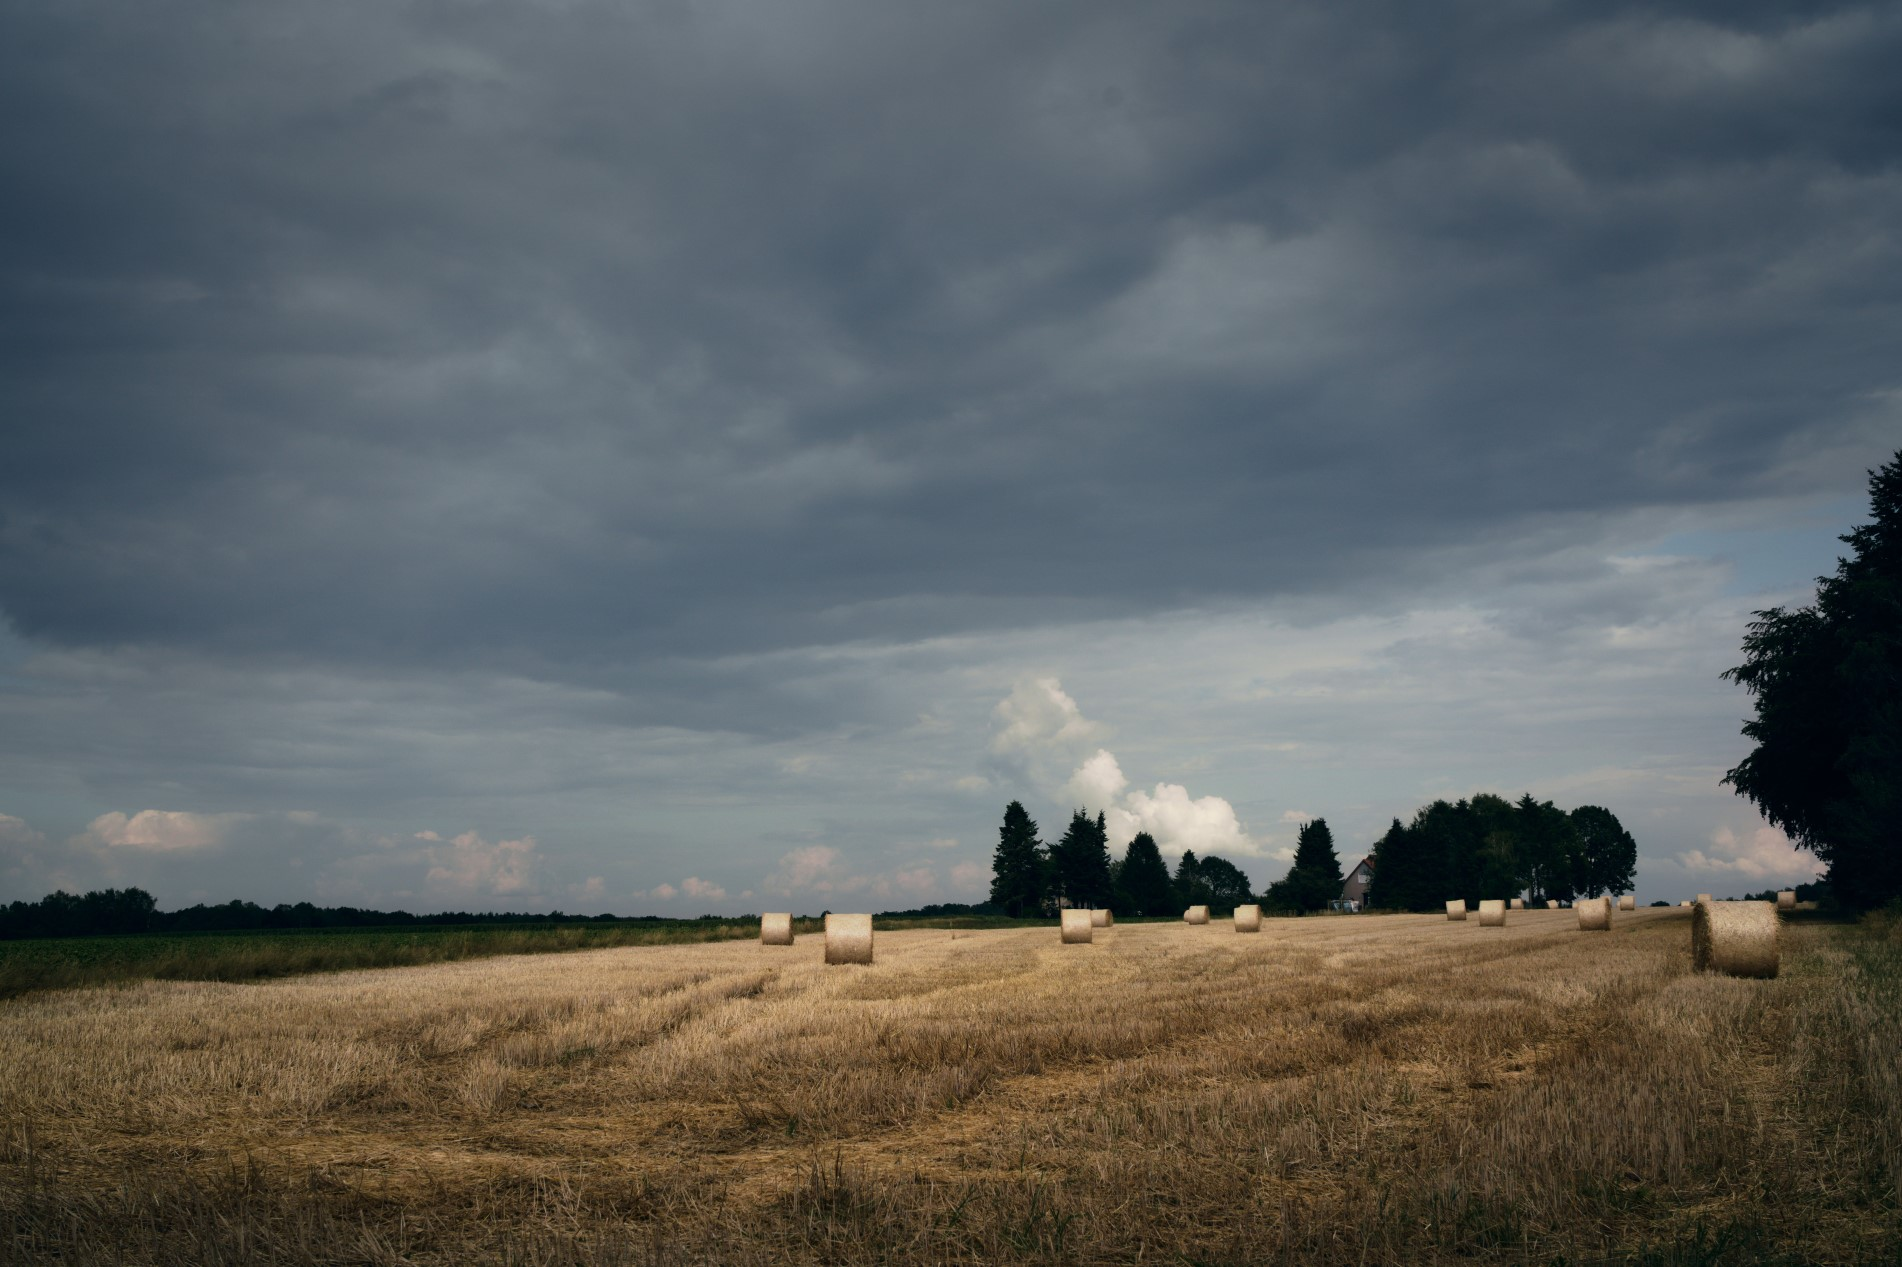
\includegraphics[width=0.7\textwidth]{field}
                    };
                    \begin{scope}[x={(image.south east)},y={(image.north west)}]

                        % All floating descriptions:
                        \foreach \x/\y/\nodetext in {
                            0.50/0.20/{A field!},
                            0.50/0.70/{The sky!}%
                        }{
                            \node at (\x,\y) {\ctrw{\nodetext}};
                        }

                        % \ctrw{} cannot deal with linebreaks contained inside of it,
                        % so it has to be applied manually each time.
                        \node[align=left, right] at (0.02, 0.50) {%
                            \ctrw{Multiple lines}\\%
                            \ctrw{with manual}\\%
                            \ctrw{linebreaks!}%
                        };%

                        \draw[annotationarrow] (0.75,0.45) -- (1.05,0.50)
                            node[align=left, right, text width=5em] {An annotation!};

                        % DEBUGGING COMMAND
                        \debugtikzsvg
                    \end{scope}
                \end{tikzpicture}
            }{
                \caption{Debugging/positioning grid}
                \label{fig:bitmap_tikz_debug}
            }%
            \vss
            \vspace{3ex}

            \ffigbox[\FBwidth]{
                \begin{tikzpicture}[%
                    every node/.style={
                        font=\footnotesize
                    }
                ]
                    \node[anchor=south west,inner sep=0] (image) at (0,0) {
                        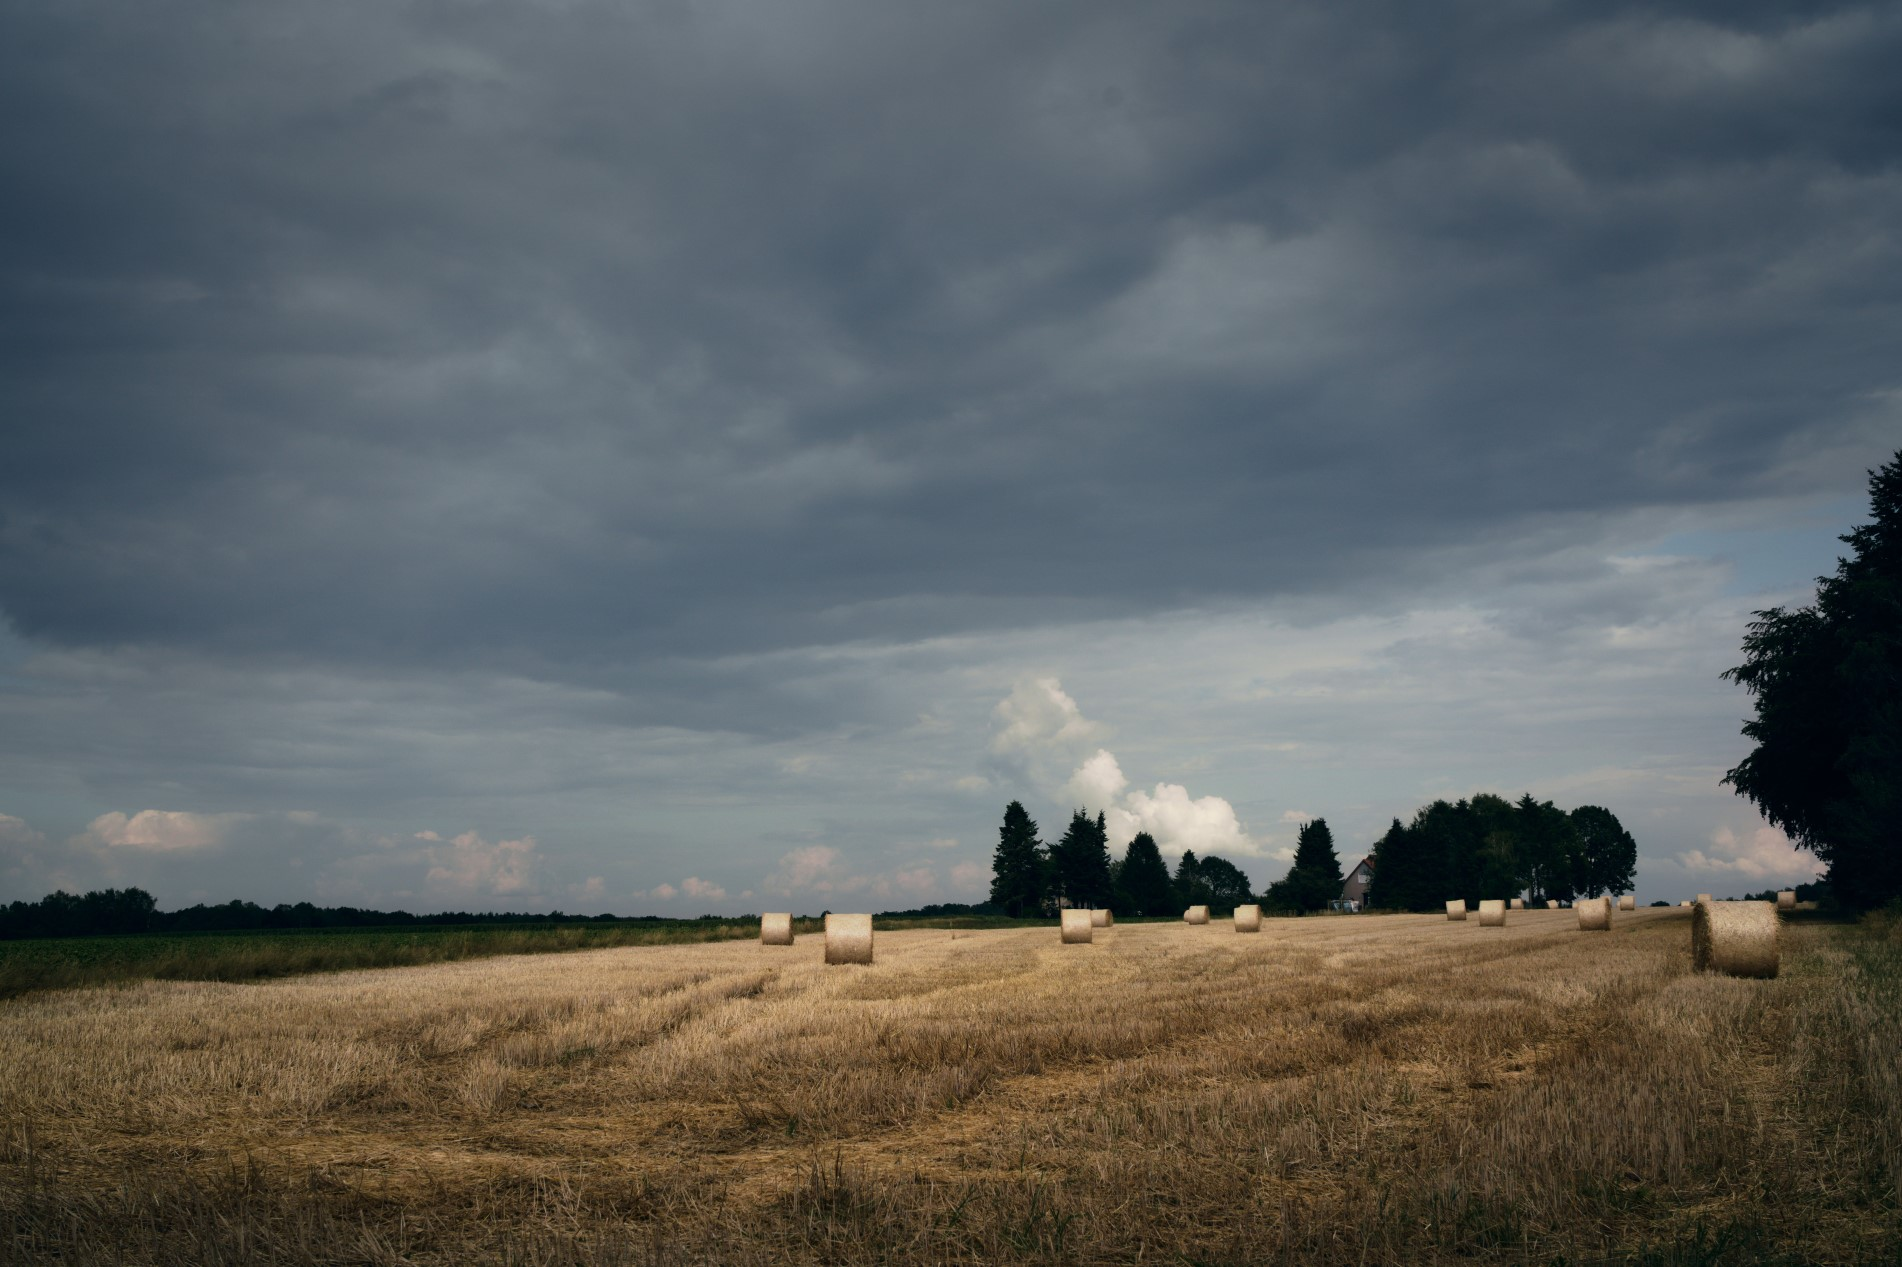
\includegraphics[width=0.7\textwidth]{field}
                    };
                    \begin{scope}[x={(image.south east)},y={(image.north west)}]

                        % All floating descriptions:
                        \foreach \x/\y/\nodetext in {
                            0.50/0.20/{A field!},
                            0.50/0.70/{The sky!}%
                        }{
                            \node at (\x,\y) {\ctrw{\nodetext}};
                        }

                        % \ctrw{} cannot deal with linebreaks contained inside of it,
                        % so it has to be applied manually each time.
                        \node[align=left, right] at (0.02, 0.50) {%
                            \ctrw{Multiple lines}\\%
                            \ctrw{with manual}\\%
                            \ctrw{linebreaks!}%
                        };%

                        \draw[annotationarrow] (0.75,0.45) -- (1.05,0.50)
                            node[align=left, right, text width=5em] {An annotation!};

                        % DEBUGGING COMMAND
                        % \debugtikzsvg
                    \end{scope}
                \end{tikzpicture}
            }{
                \caption{Result}
                \label{fig:bitmap_tikz_result}
            }
        }
        \end{subfloatrow}
    }{%
        \caption{%
            Drawing over a bitmap graphic using \idx{tikz} in a vertical sub\-/figure
            environment%
        }
        \label{fig:bitmap_tikz}
    }
\end{figure}

\subsection{Trees}

Drawing trees is possible with \ctanpackage{forest}, see \cref{fig:tree}.
It is a very easy package to get started with.
Take a look at the source code.
It is deceivingly simple, but also highly customizable.
Note that the package is stand\-/alone, but uses \idx{tikz} under the hood
(like a lot of packages do).
\begin{figure}
    \ffigbox[\textwidth]{% forest does not work with \FBwidth (?)
        \caption{Example for a tree}
        \label{fig:tree}
    }{
        \footnotesize
        \begin{forest}
            forked edges,% Instead of direct connections, draw edges
            for tree={%
                    grow'=east,
                    anchor=west,
                    where level=0{}{calign=first},% works like {if}{else}
                    %
                    % Put all nodes of same level onto same tier also, aligning
                    % them vertically:
                    tier/.pgfmath=level(),
                    %
                    where level=1{font={\bfseries}}{},%
                },%
            % Decrease distance to only affect root-first level with s sep, see
            % https://tex.stackexchange.com/a/188461/120853
            [Overall Category, anchor=south, rotate=90, for children={s sep-=1em}
                [Number One
                    [At vero eos]
                    [et accusamus]
                    [et iusto]
                ]
                [Number Two
                    [{odio dignissimos, ducimus}]% Escape commas
                    [qui blanditiis]
                    [praesentium]
                    [voluptatum]
                    [deleniti atque]
                    [corrupti quos]
                    [dolores et]
                    [quas molestias]
                ]
                [Number Three
                    [excepturi sint]
                    [occaecati]
                    [non provident]
                    [similique]
                    [sunt in culpa qui officia]
                ]
                [Number Four
                    [deserunt]
                    [mollitia
                            [{animi, id est}]
                            [laborum et]
                    ]
                ]
                [Number Four
                    [dolorum
                        [fuga]
                        [Et harum]
                    ]
                    [quidem
                        [rerum facilis]
                        [est et expedita]
                    ]
                ]
                [distinctio
                    [Nam libero]
                    [tempore]
                    [soluta nobis]
                    [est eligendi]
                ]
            ]
        \end{forest}
    }
\end{figure}

\subsection{Plotting}

If you rely on tools like \texttt{matlab2tikz}, this is for you.
Instead of these outside tools, one can plot \emph{directly} in \LaTeX{}, either
through importing external \texttt{*.csv} data (for example from experiments)
or through computing the plots using \ctanpackage{pgfplots} directly from within
\LaTeX{}.

\subsubsection{Directly in \LaTeX{}}
Plotting and computing the return values directly in \LaTeX{} is achieved through
the \texttt{declare function} command.
While the functionality is limited (owed to the limitations of \TeX{}, which is
of course not meant for this sort of thing),
it may still save a lot of time and headaches.
Finding and specifying the correct settings for \ctanpackage{pgfplots} can take
a lot of time.
This is already taken care of for this document.
As such, a plot from existing \texttt{*.csv} data can be set up in a handful of
lines using one of the built-in styles, like \texttt{regularplot}.
Plotting from a \idx{tikz} function is demonstrated in
\cref{fig:plotting_in_latex,fig:plotting_in_latex_tufte}.

\tikzset{
    declare function={% https://tex.stackexchange.com/a/279234/120853
        % SHOMATE equation for air w/ N2/O2/Ar/CO2.
        % This is needlessly complex and verbose, but showcases some interesting
        % features, like conditionals for piecewise functions.
        cpm(\x)=%
            (\x<=500) *% Below 500 degC
                (
                    0.781 *% N2
                    (
                        28.98641+1.853978*((\x+273.15)/1000)
                        -
                        9.647459*((\x+273.15)/1000)^2
                        +
                        16.63537*((\x+273.15)/1000)^3
                        +
                        0.000117/(((\x+273.15)/1000)^2)
                    )
                    +
                    0.2093 *% O2
                    (
                        31.32234-20.23531*((\x+273.15)/1000)
                        +
                        57.86644*((\x+273.15)/1000)^2
                        -
                        36.50624*((\x+273.15)/1000)^3
                        -
                        0.007374/((\x+273.15)/1000)^2
                    )
                    +
                    0.0093 *% Ar
                    (
                        20.78600+2.825911e-7*((\x+273.15)/1000)
                        -
                        1.464191e-7*((\x+273.15)/1000)^2
                        +
                        1.092131e-8*((\x+273.15)/1000)^3
                        -
                        3.661371e-8/((\x+273.15)/1000)^2
                    )
                    +
                    0.0004 *% CO2
                    (
                        24.99735+55.18696*((\x+273.15)/1000)
                        -
                        33.69137*((\x+273.15)/1000)^2
                        +
                        7.948387*((\x+273.15)/1000)^3
                        -
                        0.136638/((\x+273.15)/1000)^2
                    )
                )
            +
            (\x>500) *% Above 500 degC
                (
                    0.781 *% N2
                    (
                        19.50583+19.88705*((\x+273.15)/1000)
                        -
                        8.598535*((\x+273.15)/1000)^2
                        +
                        1.369784*((\x+273.15)/1000)^3
                        +
                        0.527691/(((\x+273.15)/1000)^2)
                    )
                    +
                    0.2093 *% O2
                    (
                        31.32234-20.23531*((\x+273.15)/1000)
                        +
                        57.86644*((\x+273.15)/1000)^2
                        -
                        36.50624*((\x+273.15)/1000)^3
                        -
                        0.007374/((\x+273.15)/1000)^2
                    )
                    +
                    0.0093 *% Ar
                    (
                        20.78600+2.825911e-7*((\x+273.15)/1000)
                        -
                        1.464191e-7*((\x+273.15)/1000)^2
                        +
                        1.092131e-8*((\x+273.15)/1000)^3
                        -
                        3.661371e-8/((\x+273.15)/1000)^2
                    )
                    +
                    0.0004 *% CO2
                    (
                        24.99735+55.18696*((\x+273.15)/1000)
                        -
                        33.69137*((\x+273.15)/1000)^2
                        +
                        7.948387*((\x+273.15)/1000)^3
                        -
                        0.136638/((\x+273.15)/1000)^2
                    )
                );
    }%
}

\begin{figure}\ContinuedFloat*
    \ffigbox[\FBwidth]{%
        \caption[Caloric parameters of air]{%
            Caloric parameters of air.
            \textbf{Avoid legends} and put info where it belongs,
            improving legibility (less back-and-forth for the eye).
            This plot is using the custom \texttt{regularplot} style%
        }%
        \label{fig:plotting_in_latex}%
    }{%
        \begin{tikzpicture}
            \begin{axis}[%
                regularplot,%
                axis y line*=right,%
                axis x line=none,%
                grid=none,% Grid can only be on one side
                % Using \ensuremath{} for each symbol, no need to use math mode here
                ylabel={\sym{ratio_of_specific_heats}},
                y unit={-},
            ]
                \addplot+[domain=20:400]{cpm(x)/(cpm(x)-8.3145)}
                    node [arrowlabel=0.3, sloped]
                        {\sym{ratio_of_specific_heats}};
            \end{axis}
            \begin{axis}[% https://tex.stackexchange.com/a/31504/120853
                regularplot,%
                xlabel={\sym{celsius_temperature}},%
                x unit={\degreeCelsius},% This is a siunitx-accepted command
                ylabel={\(\symspec{heat_capacity}_{\sym{pressure}}\)},
                y unit={\joule\per\kilogram\per\kelvin},
                cycle list shift=1,
            ]
                \addplot+[domain=20:400]{cpm(x)/0.0289524}
                    node [arrowlabel=0.3, sloped]
                        {\(\symspec{heat_capacity}_{\sym{pressure}}\)};%
            \end{axis}
        \end{tikzpicture}
    }%
\end{figure}

\begin{figure}\ContinuedFloat
    \ffigbox[\FBwidth]{%
        \caption[Tufte-like plot]{%
            Same content as \cref{fig:plotting_in_latex} in
            \enquote{\emph{\glsentryname{name.edward_tufte}}-like}
            for a modern, minimalist look where precision counts less than
            the overall message.
            For more info, refer to its namesake, \name{edward_tufte}%
        }%
        \label{fig:plotting_in_latex_tufte}
    }{%
        \begin{tikzpicture}
            \begin{axis}[%
                tuftelike,%
                ylabel={\(\symspec{heat_capacity}_{\sym{pressure}}\)},
                y unit = {\joule\per\kilogram\per\kelvin},
                xlabel={\sym{celsius_temperature}},%
                x unit = {\degreeCelsius},
                domain=50:400,
                ymin=1000,
                ymax=1100,
                ytick={1000, 1050, 1100},% Specify manually due to weird rounding
            ]
                \addplot+{cpm(x)/0.0289524}
                    node [arrowlabel=0.3, sloped]
                        {\(\symspec{heat_capacity}_{\sym{pressure}}\)};%
            \end{axis}%
            \begin{axis}[% https://tex.stackexchange.com/a/31504/120853
                tuftelike,%
                axis y line*=right,%
                axis x line=none,%
                ylabel={\sym{ratio_of_specific_heats}},%
                y unit={-},
                cycle list shift=1,
                domain= 50:400,
                ymin=1.35,
                ymax=1.4,
            ]
                \addplot+{cpm(x)/(cpm(x)-8.3145)}
                    node [arrowlabel=0.3, sloped]
                        {\sym{ratio_of_specific_heats}};
            \end{axis}
        \end{tikzpicture}
    }%
\end{figure}

\paragraph{Contour Plots}
Contour plots are too much to handle for \ctanpackage{pgfplots} itself.
This is owed to the limitations of the underlying \TeX{} engine.
What the math and computation engine of \ctanpackage{pgfplots} does is amazing,
but in the end, \TeX{} is a typesetting system, not a general\-/purpose programming
language.
However, \ctanpackage{pgfplots} has an option to delegate computations to the
external \texttt{gnuplot} tool.
In analogy to \ctanpackage{svg}, using it requires \texttt{gnuplot} itself to be
installed and on the \verb|$PATH|.
\Cref{fig:mollier_diagram} shows an example for a plot entirely specified in the
\LaTeX{} source.
All the functions required are defined using \ctanpackage{pgfplots} functionalities!
\enquote{Only} the computation itself is outsourced to \texttt{gnuplot}.
The resulting plot is two\-/dimensional, but the underlying logic is
three\-/dimensional, where one dimension was reduced, forming contours.
This is where the complexity resides.
The entire plot is just 200 lines of code, with really only half that being
lines that effectively do something useful.

\begin{figure}
    \ffigbox[\textwidth]{
        \caption[%
            \glsfmtname{name.richard_mollier} diagram for humid air as an example
            for \texttt{gnuplot}%
        ]{%
            \name{richard_mollier} diagram for humid air as an example
            for \texttt{gnuplot}.
            The entire source code required (functions \iecfeg{etc.}) is in the
            \LaTeX{} source%
        }
        \label{fig:mollier_diagram}
    }{
        \begin{tikzpicture}
            % Moving the grid lines behind our annotation nodes.
            % Else, the grid is drawn over the annotation text, which looks terrible.
            % The layer set has to be called with 'set layers' later on.
            % Code 'borrowed' from https://tex.stackexchange.com/a/456905/120853
            \pgfplotsset{
                /pgfplots/layers/Bowpark/.define layer set={
                    axis background,axis grid,main,axis ticks,axis lines,axis tick labels,
                    axis descriptions,axis foreground
                }{/pgfplots/layers/standard},
            }
            \begin{axis}[
                regularplot,
                %
                width=0.95\textwidth,
                height=0.4\textheight,
                %
                set layers=Bowpark,
                %
                every axis title/.append style={%
                    at={(0.5,1.1)},% Move above legend
                    anchor=south,%
                    font=\footnotesize%
                },
                %
                xlabel={\glsdesc{sym.moisture_content}},
                x unit={\glsunit{sym.moisture_content}},
                ylabel={Temperature},
                y unit={\degreeCelsius},
                %
                % Not displayed when viewing contour plot (view={0}{90}),
                % but maybe useful for debugging when viewing the 3d surface plot
                % at an angle
                zlabel={\glsdesc{sym.relative_humidity}},
                z unit={--},
                %
                title={% Print title depending on what ambient pressure was specified down below
                    \pgfkeys{/pgf/fpu=true}% https://tex.stackexchange.com/a/36189/120853
                    \pgfkeys{/pgf/fpu/output format=fixed}
                    \pgfmathparse{AmbientPressure/1e5}
                    %
                    For \SI[round-mode=figures, round-precision=1]{\pgfmathresult}{\bar}
                    air pressure.%
                    %
                    \pgfkeys{/pgf/fpu=false}
                },
                %
                variable=MoistureContent,% New name for default 'x' variable for unambiguity
                variable y=Temperature,% New name for default 'y' variable for unambiguity
                domain=0:20,% Moisture content range in g per kg
                domain y=-5:30,% Temperature range in degC
                %
                % Name space using 'contour/' to apply to all contour plots:
                contour/contour label style={
                    every node/.append style={text=black}
                },
                %
                % Default is 70pt. High value pushes them off to one side (HACKY;
                % see https://tex.stackexchange.com/q/443508/120853 and
                % https://tex.stackexchange.com/q/88031/120853)
                contour/label distance=10*70pt,
                %
                % point meta settings are not required for contour plotting.
                % point meta min=0,% Starting z value for color map scale
                % point meta max=1,% Ending z value for color map scale
                %
                view={0}{90},% View contour plot 'from above'
                % view={90}{0},% Debugging
                % view={0}{0},% Debugging
                %
                declare function={%
                    % No empty lines allowed in here.
                    % All equations for constant material constants like c_p.
                    %
                    AmbientPressure = 1e5;% Ambient, overall air pressure in Pascal
                    %
                    Buck(\Temperature) =
                        % Units: T in degC, Water Vapour Pressure result according
                        % to Buck in Pascal
                        611.21 * exp(
                            (18.678 - (\Temperature / 234.5) )
                            *
                            (\Temperature / (\Temperature + 257.14) )
                        );
                    %
                    Relative_Humidity(\MoistureContent,\Temperature) =
                        % Relative humidity phi as a fraction 0..1, with
                        % T (temperature) in degC and x (moisture content) in g/kg
                        AmbientPressure
                        *
                        \MoistureContent
                        /
                        (
                            1000 * (
                                Buck(\Temperature)
                                *
                                (\MoistureContent/1000 + 0.622)
                            )
                    );
                    %
                    Saturation_Moisture_Content(\Temperature) =
                        % Moisture content at saturation (phi = 1), with T in degC
                        0.622
                        *
                        Buck(\Temperature)
                        /
                        (
                            AmbientPressure - Buck(\Temperature)
                    );
                    %
                    Dry_Air_Enthalpy(\MoistureContent,\Temperature) =
                        % Enthalpy of dry air with conditional expressions, so that
                        % this is valid for both the unsaturated as well as 'foggy'
                        % (moisture content above saturation, but temperatures above
                        % freezing, so just vapour and liquid present) area
                        1.0045 * \Temperature
                        +
                        min(
                            (\MoistureContent/1000),
                            Saturation_Moisture_Content(\Temperature)
                        )
                        *
                        (
                            1.86 * \Temperature + 2500
                        )
                        +
                        max(
                            0,
                            (
                                \MoistureContent/1000
                                -
                                Saturation_Moisture_Content(\Temperature)
                            )
                        )
                        *
                        4.19 * \Temperature;
                },
            ]
                % Add the contour plots:
                \addplot3+ [
                    % surf,
                    ultra thick,
                    forget plot,% Required for legend to work
                    contour gnuplot={
                        levels={0.1, 0.5, 1},
                        draw color=rdylbu5,
                    },
                ] {Relative_Humidity(MoistureContent, Temperature)};
                \addlegendimage{color=rdylbu5, ultra thick}
                \addlegendentry{Relative Humidity}
                %
                \addplot3+ [
                    % surf,
                    ultra thick,
                    dashdotted,
                    forget plot,
                    contour gnuplot={
                        levels={20, 40, 60},
                        draw color=rdylbu2,
                    },
                ] {Dry_Air_Enthalpy(MoistureContent, Temperature)};
                %
                \addlegendimage{color=rdylbu2, ultra thick, dashdotted}
                \addlegendentry{%
                    Specific Enthalpy in \si{\kilo\joule\per\kilogram\dryair}%
                }

                % Add nodes and connect them. Connect the one we are currently
                % drawing to the previous one.
                % x and y coordinates are moisture content and temperature respectively
                \foreach [count=\i, remember=\i as \previousi]
                    \MoistureContent/\Temperature/\nodetext/\nodeorientation in {
                        1.8/3/{Ambient}/right,
                        1.8/27/{Preheated}/{above, text width=6em},
                        8.0/11/{Moisturized}/right,
                        8.0/26/{Inlet}/above,
                        9.0/21/{Room = Outlet}/{below right}%
                }{%
                    % Use edef to control node expansion within axis environment.
                    % Expand all stuff that is only present in the loop
                    \edef\temp{\noexpand\coordinate (LABELDOT_\i) at
                        (\MoistureContent, \Temperature);}
                    \temp

                    \edef\temp{\noexpand\node[
                        \nodeorientation,
                        align=center,
                        fill=white,
                        inner sep=1pt,
                        rounded corners,
                        outer sep=0.5em,
                        font=\noexpand\small
                    ] at (LABELDOT_\i) {\nodetext};}
                    \temp

                    % After the first one, start connecting backwards.
                    \ifnum \i > 1
                        \edef\temp{
                            \noexpand\draw[
                                *<-*,
                                ultra thick,
                                shorten <>={-(1.8pt + 1.4\pgflinewidth)}
                            ] (LABELDOT_\i) -- (LABELDOT_\previousi);
                        }
                        \temp
                    \fi
                }
            \end{axis}
        \end{tikzpicture}
    }
\end{figure}


\paragraph{Time-series}
Time-series plots are straightforward to implement.
\ctanpackage{pgfplots}, using its \texttt{dateplot} library, can automatically parse
and plot dates.
For this to work best and most reliably, dates and times should be in
\abb{international_organization_for_standardization} 8601 format:
\begin{center}
    \texttt{YYYY-MM-DDThh:mm:ss\phantom{Z}}:% \phantom for budget alignment

    \texttt{2020-05-19T12:15:31Z},
\end{center}
where \texttt{Z} is time\-/zone information and \texttt{T} is an arbitrary, but
fixed separator.
It can also be a simple space.
Use just the date \emph{or} time part when appropriate.

This format is unambiguous and understood worldwide as well as, most importantly here,
by computers.
No extra string and date parsing is required, it will just work in a lot of cases,
not only for \ctanpackage{pgfplots} like here.
Further, it is often the standard output format (or close to it) of measurement
equipment anyway, so there is not even a need to modify it.

An example is shown in \cref{fig:example_timeseries_plot}.
Note how the actually displayed date/time format can be modified and made human\-/readable
freely.
Only the underlying data format is best followed strictly in
\abb{international_organization_for_standardization} 8601 format.

\begin{figure}
    % Data is small enough to not require a separate CSV file, put it here.
    % Specify date as YYYY-MM-DD for pgfplots to recognize it as date data automatically.
    % Currently, the xlabel alignment is off using dateplots, so revert to plain
    % old methods for now.
    \pgfplotstableread[row sep=\\]{%
        Date, Apples, Bananas, Peaches, Kiwis, Skunks, Grapes, Lemons\\%
        2020-02-01, 50, 1, 17, 10, 15, 2, 5\\%
        2020-03-04, 40, 2, 32, 10, 10, 2, 4\\%
        2020-05-02, 30, 3, 37, 10, 15, 2, 3\\%
        2020-05-28, 20, 4, 52, 10, 10, 2, 2\\%
        2020-06-14, 10, 5, 57, 10, 15, 2, 1\\%
    }{\examplepfgtable}%
    %
    \ffigbox[\FBwidth]{
        \caption[Example automatic timeseries plot]{
            Example automatic timeseries plot.
            Note the automatic spacing\-/out according to the actual time deltas,
            and the automatic conversion of timestamps to human\-/friendly versions,
            to whatever specification the author chooses.
            Also note the colors: here, \emph{distinction} is important and a
            \emph{qualitative} palette is chosen.
            A \emph{sequential} or a \emph{diverging} palette would have been
            less suited (some would say plain wrong)%
        }%
        \label{fig:example_timeseries_plot}%
    }{%
        \begin{tikzpicture}
            \begin{axis}[%
                    regularplot,
                    width=0.9\textwidth,
                    height=0.3\textheight,
                    ybar stacked,
                    xtick=data,% xticks at data points, not uniformly
                    % Use next line for manual labels from table; get from {<table>}{<column>}
                    % xticklabels from table={\examplepfgtable}{year},
                    %
                    % If using date data in the table (of the form YYYY-MM-DD):
                    date coordinates in=x,
                    %
                    % Customize display here; macros automatically defined/grabbed
                    % by pgfplots:
                    xticklabel={\day.\month.\year},
                    %
                    xticklabel style={rotate=45,anchor=north east},
                    ymin=0,% Cuts off data otherwise
                    ylabel={Share},
                    y unit={\percent},
                    xlabel={Date of purchase},
                    legend style={font=\scriptsize},%
                    % nodes near coords,% uncomment for numeric labels
                    cycle list/Set2-7,
                    every axis plot/.append style={fill},% https://tex.stackexchange.com/a/317684/120853
                ]
                \foreach \columnname in {Apples, Bananas, Peaches, Kiwis, Skunks, Grapes, Lemons}{%
                    \addplot+ table [y=\columnname] {\examplepfgtable};
                }
                % Legend manually; \addlegenentry per \foreach loop is very error-prone
                \legend{Apples, Bananas, Peaches, Kiwis, Skunks, Grapes, Lemons}
            \end{axis}
        \end{tikzpicture}
    }
\end{figure}


\subsubsection{Importing CSV}

Often, one wants to plot data from files.
The better behaved the file is (meaningful headers, no junk rows), the easier that is.
In \cref{fig:diffuser}, \verb|y=<column header>| is all that has to be specified for the
column corresponding to that name to be automatically chosen, with no confusion
about indices or column numbers.
\begin{figure}
\ffigbox[\FBwidth]{
        \caption{Plotting from CSV data for a diffuser}
        \label{fig:diffuser}
    }{%
        \pgfplotstableread{data/diffuser.csv}{\diffusertable}%
        \begin{tikzpicture}
            \begin{axis}[%
                tuftelike,%
                axis y line*=left,%
                xlabel={\(\sym{radius}/\sym{radius}_{\num{2}}\)},%
                x unit={-},
                ylabel={
                    \sym{mach_number},
                    \(\sym{pressure}/\sym{pressure}_{\num{2}}\),
                    \(\sym{abs_temperature}/\sym{abs_temperature}_{\num{2}}\),
                    \(\sym{density}/\sym{density}_{\num{2}}\)
                },%
                y unit={-},
                table/x={R_pres},%
                ymin=0.4,
                ymax=1.3,
                ytick={0.4, 0.7, 1, 1.3},
                xmin=1,
                xmax=1.6
            ]%
                % Do this manually, node macro expansion in foreach/invokeforeach
                % is error-prone
                \addplot+ table [y=M] {\diffusertable}
                    node [arrowlabel=0.2]
                    {\sym{mach_number}};
                \addplot+ table [y=Pi] {\diffusertable}
                    node [arrowlabel=0.9]
                    {\(\sym{pressure}/\sym{pressure}_{\num{2}}\)};
                \addplot+ table [y=Theta] {\diffusertable}
                    node [arrowlabel=0.7]
                    {\(\sym{abs_temperature}/\sym{abs_temperature}_{\num{2}}\)};
                \addplot+ table [y=Rho] {\diffusertable}
                    node [arrowlabel=0.8]
                    {\(\sym{density}/\sym{density}_{\num{2}}\)};
            \end{axis}%
            %
            \begin{axis}[%
                tuftelike,%
                axis y line*=right,%
                axis x line=none,%
                ylabel={abs.\ flow angle \sym{angle_one}},%
                y unit={\degree},
                cycle list shift=4,%
                ymin=13,
                ymax=15,
                xmin=1,
                xmax=1.6,
            ]%
                \addplot+ table [x=R_pres, y=alpha] {\diffusertable}
                    node [arrowlabel] {\sym{angle_one}};%
            \end{axis}%
        \end{tikzpicture}
    }
\end{figure}

\subsubsection{Using MATLAB2Ti\textit{k}Z}

\href{https://github.com/matlab2tikz/matlab2tikz}{MATLAB2Ti\textit{k}Z} is a tool to
convert MATLAB figures to \LaTeX{}, see \cref{fig:matlab2tikz}.
Notice that by default, it exports using whitespace (tabs) as column separators,
which might differ from what you set as a global option in \verb|\pgfplotstableset|.

\begin{figure}
    \ffigbox[\FBwidth]{%
        \caption[%
            A vanilla \href{https://github.com/matlab2tikz/matlab2tikz}{MATLAB2Ti\textit{k}Z}
            example%
        ]{%
            A vanilla \href{https://github.com/matlab2tikz/matlab2tikz}{MATLAB2Ti\textit{k}Z}
            example, imported here without changes except those to allow successful compilation
            (see commit \texttt{56556a0}: set \texttt{table/col sep=space}).
            While it works, the style created in MATLAB conflicts with the local one,
            and you miss out on many useful features, like \ctanpackage{siunitx} or
            \ctanpackage{glossaries-extra}.
            A more frictionless approach is to export plain-text (CSV) data from MATLAB,
            and import it into \LaTeX{}, see \cref{fig:diffuser}%
        }%
        \label{fig:matlab2tikz}%
    }{%
        % Can't use `subimport', since import is not from any child directory.
        \import{data/}{matlab2tikz_table_example}
    }
\end{figure}

\subsection{TikZ and Text}

\idx{tikz} content can also be intertwined with text using \verb|\tikzmark|.
This is illustrated in \cref{eq:tikz_in_text}.
Note that this procedure needs two compilation runs, since the label positions
need to be written to an auxiliary file first.

\begin{minipage}{1\linewidth}
    % https://tex.stackexchange.com/q/83746/120853 and
    % https://tex.stackexchange.com/a/188221/120853
    \newcommand*{\setmuskip}[2]{#1=#2\relax}
    \setmuskip{\medmuskip}{15mu plus 2mu minus 4mu}
    \setmuskip{\thickmuskip}{18mu plus 2mu minus 4mu}

    \begin{equation}\label{eq:tikz_in_text}
        \tikzmark{c}\sym{mass_fraction}_{\chcpd{C}}
        +
        \tikzmark{h}\sym{mass_fraction}_{\chcpd{H}}
        +
        \tikzmark{s}\sym{mass_fraction}_{\chcpd{S}}
        +
        \tikzmark{o}\sym{mass_fraction}_{\chcpd{O}}
        +
        \tikzmark{n}\sym{mass_fraction}_{\chcpd{N}}
        +
        \tikzmark{w}\sym{mass_fraction}_{\chcpd{H2O}}
        +
        \tikzmark{a}\sym{mass_fraction}_{\mathrm{ash}}
        \coloneq% prints as :=
        \num{1}
        \eqend{}
    \end{equation}

    \begin{tikzpicture}[%
        remember picture,%
        overlay,%
    ]
        \pgfmathsetmacro{\vshiftone}{4}
        \pgfmathsetmacro{\vshifttwo}{6.5}
        \pgfmathsetmacro{\vshiftthree}{9}
        \pgfmathsetmacro{\hshiftone}{1}
        \pgfmathsetmacro{\hshifttwo}{2}
        \pgfmathsetmacro{\hshiftthree}{3}

        \foreach \x/\y/\a/\b in {%
            c/Carbon/\vshiftone/-\hshiftthree,%
            h/Hydrogen/\vshifttwo/-\hshifttwo,%
            s/Sulphur/\vshiftthree/-\hshiftone,%
            o/Oxygen/\vshifttwo/0,%
            n/Nitrogen/\vshiftthree/\hshiftone,%
            w/Water/\vshifttwo/\hshifttwo,%
            a/Ash/\vshiftone/\hshiftthree%
        }{%
            \node (\x1) [below right=0.1em and 0.4em of pic cs:\x]
                {};
            \node (\x2) [on grid, below right=\a ex and \b ex of \x1, anchor=north]
                % 'on grid' option makes positioning snappy (uses actual middle
                % of nodes); without, even 'right=0pt' would not be centered
                {\y};
            \draw[-stealth] [out=90](\x2) to [in=270](\x1);
        }%
    \end{tikzpicture}

    % We need to use 'overlay', but this also means we lose the bounding box.
    % Eye-ball it here, sadly.
    \vspace{4\baselineskip}
\end{minipage}

\subsection{Regular TikZ pictures}

\idx{tikz} really is not meant for arbitrary graphics.
The more free\-/form images shown in this document were created using InkScape.
Still, \enquote{drawing} in \idx{tikz} is much preferred and easier when the
images are somewhat programmatic, aka there are straight corners, edges and turns,
equal distances, and everything is a bit \enquote{block-like}, repetitive.
For example, a small file structure diagram:
\begin{center}
    \begin{tikzpicture}[
        %http://www.texample.net/tikz/examples/filesystem-tree/
            grow via three points={one child at (0.5,-0.7) and
                two children at (0.5,-0.7) and (0.5,-1.4)},
            edge from parent path={(\tikzparentnode.south) |- (\tikzchildnode.west)},
            every node/.style={draw=black,thick,anchor=west,fill=g5},
            font=\ttfamily,%
        ]%
            \node {\faFileO{} parent.py}
            child { node {\faFileO{} constants.py}}
            child { node {\faFileO{} parameters.py}}
            child { node {\faFileO{} handling.py}}
            child { node {\faFileO{} performance\_maps.py}};
    \end{tikzpicture}
\end{center}
Note how \verb|tikzpicture| environments do not have to be contained in floats.

More \idx{tikz} examples are shown in
\cref{fig:tikz_control_diagram,fig:tikz_circuit_example,fig:tikz_threedimensional_example}.

\begin{figure}\ContinuedFloat*
    \ffigbox[0.95\linewidth]{%
        \begin{tikzpicture}[%
            every path/.style={thick},%https://tex.stackexchange.com/a/302931/120853
            simblock/.style={%
                draw,%
                line width=1.5pt,%
                minimum size=1.5em,%
                rounded corners,%
                fill=white,%
            },%
            triangle/.style={%
                regular polygon,%
                regular polygon sides=3,%
                inner sep=0.2ex,% Fit tightly
                outer sep=0pt,
            },
        ]%
        % Row of Model Blocks
            \node[simblock, minimum height=5ex] (outlet)
                {Outlet};
            \node[simblock, minimum height=5ex, right=of outlet] (turbine)
                {Turbine};
            \node[simblock, minimum height=5ex, right=of turbine] (compressor)
                {Compressor};
            \node[simblock, minimum height=5ex, right=of compressor] (inlet)
                {Inlet};
            \draw[->] (outlet) -- (turbine)
                node [midway, above, font=\footnotesize] {feeds};
            \draw[->] (turbine) -- (compressor)
                node [midway, above, font=\footnotesize, align=center] (shaft) {via\\shaft};
            \draw[->] (compressor) -- (inlet)
                node [midway, above, font=\footnotesize] {feeds};

            % Division Block underneath Engine
            \node[below=12ex of inlet.south, draw=none] (div) {};
            \node[below=4ex of div, draw=none] (mult) {};
            \node[simblock, fit=(mult) (div), minimum height=8ex] (multdiv) {};
            \node at (div) {\(\div\)};
            \node at (mult) {\(\ast\)};

            % Connect Inlet and Division part
            \draw[->] (inlet.east) -- ++ (+1, 0)
                node [pos=1, above] {\(p_{\text{in}}(\tau)\)}
                |-
                ($(multdiv.east)!0.5!(multdiv.north east)$);

            % p min block next to multiplication
            \draw[<-] ($(multdiv.east)!0.5!(multdiv.south east)$) -- ++ (1, 0)
                node[simblock] {\(p\)};

            \node [circle, fill, inner sep=0.3ex, left=0.7em of multdiv] (split1) {};
            \draw (multdiv) -- (split1);

            % Bias and inverted Bias blocks
            \node[simblock, left = of div] (biasinv) {\(1 - u\)};
            \node[simblock, left = of mult] (bias) {\(u - 1\)};
            \draw[->] (split1) |- (bias);
            \draw[->] (split1) |- (biasinv);

            % Split again
            \node [circle, fill, inner sep=0.3ex, left=1em of biasinv] (split2) {};
            \draw (biasinv) -- (split2);

            \node[simblock, left=1em of split2, triangle, shape border rotate=90] (gainint)
                {\small\(I\)};
            \draw[->] (split2) -- (gainint);

            \node[simblock, above=of gainint, triangle, shape border rotate=90] (gainp)
                {\small\(P\)};
            \draw[->] (split2) |- (gainp);

            % Intersection between Integer Gain and Multi/Div block as helper
            \coordinate (help1) at (gainint|-multdiv);

            % Integer Text, but don't draw
            \node[draw=none, left=4em of help1, minimum height=8ex] (int)
                {\(\frac{KTs}{z - 1}\)};

            % Falling Edge Sign with Arrow
            \draw ($(int.east)!0.5!(int.south east)$)
                -- ++ (0.5em, 0)
                -- ++ (0, -0.7em)
                -- ++ (0.5em, 0) coordinate (intsign_end);
            \draw[thin, ->] ($(int.east)!0.5!(int.south east)$)
                -- ++ (0.5em, 0) -- ++ (0, -0.5em);

            % Move fitting to background so it does not overwrite the nodes it fits to
            \begin{pgfonlayer}{background}
                \node[simblock, fit=(int.north west)(intsign_end)] (int_block) {};
            \end{pgfonlayer}

            \draw[->] (bias) -- (int_block.east|-mult)
                node [midway, below, align=center, font=\footnotesize]
                    {falling edge\\reset};
            \draw[->] (gainint) -- (int_block.east|-div);

            \node [simblock, circle, left=of int_block] (sum) {};
            \draw[->] (gainp) -| (sum) node [pos = 0.9, right] {\(+\)};
            \draw[->] (int_block) -- (sum) node [pos = 0.8, below] {\(+\)};

            \node[simblock, left = of sum] (biasinvout) {\(1- u\)};
            \draw[->] (sum) -- (biasinvout);

            \node[simblock, left = of outlet] (times) {\(\times\)};
            \draw[->] (times) -- (outlet) node [midway, above, font=\footnotesize]
                {\(\dot{\sym{mass}}_{\text{T}}\)};

            \node[simblock, below=of times] (sat) {\(\num{0.1} \leq u \leq \num{1}\)};
            \draw[->] (biasinvout) -| (sat);
            \draw[->] (sat) -- (times) node [midway, left]
                {\(\symbf{\zeta(\tau)}\)};

            \node[simblock, above=of outlet, minimum height=5ex] (eng) {Engine};

            \draw[->] (inlet) |- (eng) node [pos=0.8, above, font=\footnotesize]
                {feeds};
            \draw[->] (eng) -| (times) node [pos=0.7, left, font=\footnotesize]
                {\(\dot{\sym{mass}}_{\text{E}}\)};
        \end{tikzpicture}
    }{%
        \caption[Wastegate implementation in a feedback\-/loop]{%
            % See here: https://tex.stackexchange.com/a/471263/120853
            % for a good macro to print "MATLAB/Simulink" (not used here since it
            % it wouldn't be used much at all)
            Wastegate implementation in a feedback\-/loop in MATLAB/Simulink
            as an example for a \idx{tikz} diagram%
        }%
        \label{fig:tikz_control_diagram}%
    }%
\end{figure}

\begin{figure}\ContinuedFloat
    \fcapside[\FBwidth]{
        \caption{Example for the \texttt{circuits.ee.IEC} \idx{tikz} library}
        \label{fig:tikz_circuit_example}
    }{
        \begin{tikzpicture}[
                circuit ee IEC,% As loaded by the lib of the same name
                % every circuit symbol/.style={thick},
            ]
            \pgfmathsetmacro{\circuitwidth}{4}
            \pgfmathsetmacro{\circuitheight}{2}
            % Try to close manually, we cannot 'cycle'
            % https://tex.stackexchange.com/q/33294/120853
            \draw (0,0) -- node[contact] (CONTACT_LEFT) {} (0,\circuitheight)
                to [resistor={name={RESISTOR}, info={\sym{electrical_resistance}}}]
                    node[%
                        current direction,
                        pos=0.9,
                        label={[name=ELECTRIC_CURRENT_LABEL]above:{\(\sym{electric_current}\)}}
                    ] {}
                (\circuitwidth,\circuitheight) -- node[contact] (CONTACT_RIGHT) {}
                (\circuitwidth,0) to [battery] (0,0);

            \draw[<->, shorten <>=0.7em] (CONTACT_LEFT) -- (CONTACT_RIGHT)
                node[arrowlabel] {\(\sym{voltage}\)};

            \node[
                fit={(RESISTOR)(ELECTRIC_CURRENT_LABEL)(CONTACT_LEFT)(CONTACT_RIGHT)},
                inner sep=1em,
                draw,
                dashed
            ] (BOUNDARY) {};

            % The following draws a label directly onto the node border.
            % Cannot really be done with supplying a 'label' directly to the node
            % BOUNDARY (?)
            \node[fill=white, font={\small}] at (BOUNDARY.north) {Boundary};
        \end{tikzpicture}
    }
\end{figure}

\begin{figure}\ContinuedFloat
    \fcapside[\FBwidth]{
        \caption{%
            Example for a three\-/dimensional \idx{tikz} drawing using the
            \texttt{3d} library%
        }
        \label{fig:tikz_threedimensional_example}
    }{
        \tdplotsetmaincoords{110}{-12}% View angle
        \begin{tikzpicture}[tdplot_main_coords]
            % Debugging coordinate system:
            % \draw (0,0,0) -- (1,0,0) node[right] {\(x\)};
            % \draw (0,0,0) -- (0,1,0) node[left] {\(y\)};
            % \draw (0,0,0) -- (0,0,1) node[above] {\(z\)};

            % Base measurements. Default unit is centimeter
            \pgfmathsetmacro{\plateheight}{0.2}
            \pgfmathsetmacro{\platewidth}{4}
            \pgfmathsetmacro{\platedepth}{3}
            % Stretch how arrows are distanced from the plate:
            \pgfmathsetmacro{\arrowdistance}{2.5}

            % Bottom arrow:
            \begin{scope}[canvas is xy plane at z=-\plateheight/\arrowdistance]
                \draw[flowarrow={4em}{0.2em}, solid] (-\platewidth*0.25,\platedepth*0.5)
                    node[left] {\(\flow{\sym{mass}}_{2}''\)}
                    --
                    (\platewidth*1.25,\platedepth*0.5)
                    node[right] {\(\flow{\sym{mass}}_{2}'\)};
            \end{scope}

            % Top surface:
            \begin{scope}[canvas is xy plane at z=\plateheight]
                \draw[wall] (0,0) rectangle (\platewidth,\platedepth)
                    node[midway] {\ctrw{\(\sym{area}\)}};
            \end{scope}
            % Right surface:
            \begin{scope}[canvas is yz plane at x=\platewidth]
                \draw[wall] (0,0) rectangle (\platedepth,\plateheight);
            \end{scope}
            % Front surface:
            \begin{scope}[canvas is xz plane at y=\platedepth]
                \draw[wall] (0,0) rectangle (\platewidth,\plateheight);

                \foreach [count=\i] \posfraction in {0.2, 0.4, ..., 0.8}{%
                    \draw[->, dashed, thick] (\posfraction*\platewidth, \plateheight*2)
                    --
                    (\posfraction*\platewidth, -2*\plateheight) coordinate[below] (ARROW_\i);
                }
            \end{scope}

            % Top arrow:
            \begin{scope}[canvas is xy plane at z=\plateheight*\arrowdistance]
                \draw[flowarrow={4em}{0.2em}, solid] (\platewidth*1.25,\platedepth*0.5)
                    node[right] {\(\flow{\sym{mass}}_{1}''\)}
                    --
                    (-\platewidth*0.25,\platedepth*0.5)
                    node[left] {\(\flow{\sym{mass}}_{1}'\)};
            \end{scope}

            % Manually set arrow label here:
            \node at ($(ARROW_1)!0.5!(ARROW_4)$) {\(\flow{\sym{volume}}\)};
        \end{tikzpicture}
    }
\end{figure}

\paragraph{Included shapes}
This repository includes custom\-/made shapes for thermodynamic applications.
These can be used like many other \idx{tikz} elements, for example by
positioning them somewhere on the canvas, connecting them to other elements,
rotating them \iecfeg{etc}.
In that sense, they work like usual \idx{tikz} elements (just buggier\dots{}).
There are a couple of advantages:
\begin{enumerate}
    \item unified looks: no more drawing these in InkScape, where they come out
        slightly dissimilar every time,
    \item tight integration with \idx{tikz}, allowing to use all its other
        features,
    \item very fast generation of drawings once some familiarity is gained;
        with InkScape or other outside tools, one can also become fast, but it is
        hard to beat a \LaTeX{}\-/internal approach.
\end{enumerate}
Examples are shown in
\cref{fig:tikz_thermodynamic_drawing,fig:tikz_thermodynamics_radiators}.
Refer to their source code to see how more or less easily they are created.

\begin{figure}\ContinuedFloat*
    \ffigbox[\FBwidth]{
        \caption{%
            Example for a thermodynamic device drawing using \idx{tikz}.
            It relies heavily on the custom\-/made library of shapes%
        }
        \label{fig:tikz_thermodynamic_drawing}
    }{
        \begin{tikzpicture}[
            thisshaft/.style={
                line width=3pt
            },
            every label/.style={
                font=\footnotesize
            },
            every node/.style={
                font=\footnotesize
            }
        ]
            % The main circle itself:
            % Note that when rotating shapes, the label positions also rotate and get mixed up.
            \draw (0,0) --
                node[midway, valve, sloped, label=left:Throttle] (VALVE) {} (0,2.5) --
                node[midway, heat exchanger, rotate=180, label=above:Condenser] (CONDENSER) {} (5,2.5) --
                (5,0)
                node[midway, compressor, label=above:Compressor, rotate=180] (COMPRESSOR) {} --
                node[midway, heat exchanger, label=above:Evaporator] (EVAPORATOR) {}
                cycle;

            % Engine on right of compressor:
            \draw[thisshaft] (COMPRESSOR) -- ++ (2,0)
                node [right, rectangle, draw, thin] (ENGINE) {Engine}
                    coordinate[midway] (SHAFT_MIDDLE);

            % Shift down by 7pt (shaft line width is 3pt) and also specify that as a radius
            \draw[->] ([yshift=-7pt]SHAFT_MIDDLE) arc (290:60:7pt);

            \foreach [count=\i] \xcomponent/\ycomponent/\orientation in {
                COMPRESSOR/EVAPORATOR/right,
                COMPRESSOR/CONDENSER/right,
                VALVE/CONDENSER/left,
                VALVE/EVAPORATOR/left%
            }{
                \node[
                    origindot,
                    label={[name={NUMBER_\i}]\orientation:{\num{\i}}}
                ] at (\xcomponent|-\ycomponent) {};
            }

            \draw[<-] (EVAPORATOR) -- ++ (0,-0.8)
                node[at end, below, align=center]
                    {supplied heat} coordinate[near start] (LOWER_BOUNDARY);

            \draw[->] (CONDENSER) -- ++ (0,1.2) coordinate[pos=0.6] (UPPER_BOUNDARY)
                node[at end, above, align=center]
                    {heat discharge} coordinate[near start] (A);

            % Drawings around engine
            \draw[->, dashdotted] (ENGINE) |-
                node[very near end, right, fill=white] {excess engine heat} (A);
            \draw[<-] (ENGINE) -- ++ (1.3,0) node[right, align=left]
                {Electricity,\\gas} coordinate[midway] (RIGHT_BOUNDARY);

            % Fit a rectangle around the relevant parts:
            \node[
                fit={(UPPER_BOUNDARY)(LOWER_BOUNDARY)(RIGHT_BOUNDARY)(VALVE)(NUMBER_3)(NUMBER_4)},
                draw,
                dashed
            ] (COP_BOUNDARY) {};

            % COP area labels.
            \node[fill=white, left] at ([xshift=-2em]COP_BOUNDARY.north east)
                {\glsxtrshort{abb.coefficient_of_performance}-Boundary};
        \end{tikzpicture}
    }
\end{figure}

\begin{figure}\ContinuedFloat
    \tikzset{
        thispipe/.style={rounded corners=0.5},
        node distance=1em,
        every node/.style={font=\small}
    }
    \ffigbox[\FBwidth]{%
        \caption{Example \idx{tikz} shapes}
        \label{fig:tikz_thermodynamics_radiators}
    }{%
        \begin{tikzpicture}
            \pgfmathsetmacro{\gridspread}{2.2}
            \pgfmathsetmacro{\numberofrows}{3}
            \pgfmathsetmacro{\numberofcolumns}{3}
            % Extension by which the pipes expand to the left, out of the radiators:
            \pgfmathsetmacro{\pipeextension}{1}

            \foreach [remember=\x as \prevx] \x in {1, 2, ..., \numberofcolumns}{
                    \foreach [remember=\y as \prevy] \y in {1, 2, ..., \numberofrows}{
                            \node[radiator] at (\x*\gridspread, 0.7*\y*\gridspread) (RADIATOR_\x_\y) {};

                            % Draw the radiators with pipes sticking out:
                            % \ifnum doesn't have elseif, so nest if
                            \ifnum \x = 1
                                \draw[thispipe] (RADIATOR_\x_\y.upper entry) -- ++
                                    (-\pipeextension, 0) node[midway, control valve] {}
                                    node[at end, origindot] (UPPER_PIPE_END_\x_\y) {};
                                \draw[thispipe] (RADIATOR_\x_\y.lower entry) --
                                    (RADIATOR_\x_\y.lower entry-|UPPER_PIPE_END_\x_\y)
                                    node[at end, origindot] (LOWER_PIPE_END_\x_\y) {};
                                % Connect the two pipe ends:
                                \draw[thispipe] (UPPER_PIPE_END_\x_\y) -- (LOWER_PIPE_END_\x_\y);
                            \else
                                \ifnum \x = 2
                                    \draw[thispipe] (RADIATOR_\x_\y.upper entry) -- ++
                                        (-0.4*\pipeextension, 0)
                                        node[at end, threeway valve, rotate=-90] (THREEWAY_VALVE_\x_\y) {};
                                    \draw[thispipe] (RADIATOR_\x_\y.lower entry) --
                                        (RADIATOR_\x_\y.lower entry-|THREEWAY_VALVE_\x_\y.south)
                                        node[at end, origindot] (LOWER_PIPE_END_\x_\y) {};
                                    % Connect valve to lower pipe end:
                                    \draw[thispipe] (THREEWAY_VALVE_\x_\y.south) --
                                        (LOWER_PIPE_END_\x_\y);
                                    % Create an alias for this row, since pipe end is now at threeway valve north input.
                                    % This way, we can use it like the other ones at the bottom.
                                    \coordinate (UPPER_PIPE_END_\x_\y) at (THREEWAY_VALVE_\x_\y.north);
                                \else% In all other cases, so the rows after the second to the right
                                    % Upper radiator entry to the left:
                                    \draw[thispipe] (RADIATOR_\x_\y.upper entry) -- ++
                                        (-0.2*\pipeextension, 0) coordinate[at end] (UPPER_PIPE_END_\x_\y);
                                    % Lower radiator entry to the left:
                                    \draw[thispipe] (RADIATOR_\x_\y.lower entry) --
                                        (RADIATOR_\x_\y.lower entry-|UPPER_PIPE_END_\x_\y)
                                            coordinate[at end] (LOWER_PIPE_END_\x_\y);
                                \fi
                            \fi
                            % After the first row, connect radiator pipes to the previous ones:
                            \ifnum \y > 1
                                \draw (UPPER_PIPE_END_\x_\prevy) -- (LOWER_PIPE_END_\x_\y);
                            \fi
                        }
                }

            \pic[below left=0em and 3em of LOWER_PIPE_END_1_1, scale=0.3, pic text={Boiler}]
                (BOILER) {boiler};

            % Helper coordinates because perpendicularity operator (-| or |-) seems to have trouble in conjunction with calculated nodes ($ $)
            \coordinate (BOILERTOP) at ($(BOILER.before top)!0.5!(BOILER.after top)$);
            % Pipe from boiler straight up, until criteration is met:
            \draw[thispipe] (BOILERTOP) --
                ([yshift=1.5em]BOILERTOP|-UPPER_PIPE_END_1_\numberofrows)
                coordinate[at end] (BOILER_OUT_PIPE_END)
                node[pos=0.2, pump] {};

            \foreach \x in {1, 2, ..., \numberofcolumns}{
                    % Connect end of boiler vertical pipe to each radiator column:
                    \draw[thispipe] (BOILER_OUT_PIPE_END) -|
                        (UPPER_PIPE_END_\x_\numberofrows);
                    % Connect bottom row lower pipes to boiler:
                    \draw[thispipe, ->] (LOWER_PIPE_END_\x_1) |- (BOILER.east);
                }

            % Helper coords to make calc etc work reliably
            \coordinate (B) at (BOILER.east-|LOWER_PIPE_END_1_1);
            \coordinate (EQUALIZING_TANK_PIPE_POSITION) at ($(B)!0.5!(BOILER.east)$);

            % Set it above horizontal middle of boiler and start of first row.
            \draw (EQUALIZING_TANK_PIPE_POSITION) -- ++ (0, 2em) node[equalizing tank] {};

            % 'Air discharged (Lufttopf)' at top
            \draw[thispipe] (BOILER_OUT_PIPE_END) -- ++ (0, 0.5em)
                node[
                    at end,
                    rectangle,
                    draw,
                    minimum width=1em,
                    minimum height=1.5em,
                    anchor=south,
                    label=right:{Air Discharge}
                ] (AIR_DISCHARGE) {};
            \draw[thispipe, ->] (AIR_DISCHARGE.north) -- ++ (0, 0.75em) -|
                ([shift={(0.5em, 0.75em)}]AIR_DISCHARGE.east);
        \end{tikzpicture}
    }
\end{figure}

\subsection{InkScape}

Having seen what \idx{tikz} is good at,
\cref{fig:tighter_caption,fig:multiple_floats,fig:sidecap}
are good examples for when InkScape might be the better choice:
three\-/dimensional, curvy drawings.

\Cref{fig:tighter_caption} is a vectorized bitmap.
InkScape can detect edges and contrasts in bitmaps and replicate those lines in
vector format (\texttt{Path > Trace Bitmap}).

\section{Example Boxes}

As a special gimmick, there is an environment for examples (can also be renamed).
It may be useless now, but you can alter it to suit your needs; the skeleton is
there for you.
It even has its own list, like the list of figures.
For an example box, see \cref{ex:example}.

\begin{example}[%
    label={ex:example},%
]{%
    I am a useless box%
}
    There can be pretty much any content in here.
    Math works --- as we can see,
    \begin{equation}
        1 = 1
    \end{equation}
    still holds true after all these years!

    If the \verb|float| setting is set, this box also floats.
    Inserting other floats in here will then cause \LaTeX{} to have a massive fit
    (floats inside floats do not make sense).
    This is circumvented setting the \verb|[H]| flag,
    saying \enquote{this float is not really a float, pin it down \emph{right} here}.

    \textbf{In any other context, setting any such flag is code smell/poor style.}
    These are often used wrong and just as often set prematurely and then reset
    countless times, all the while \LaTeX{} complains (rightfully so) about the poor
    spacing introduced by forcing float positions, instead of letting \LaTeX{} take
    care of it.
    For the love of God, let \LaTeX{} do its job in placing the floats.
    Truth be told, they will on occasion not be placed where you need or want them.
    Keep working.
    At the very end, when all is done, go ahead and change the few \emph{truly}
    misplaced floats manually, by shoving them about in the source code
    (still not using \verb|htb!| flags).
    This ensures minimal pain and maximum usage of \LaTeX{}'s spacing and placing
    capabilities.

    Anyway --- here is such a float within an example box:
    \begin{figure}[H]
        \fcapside[\FBwidth]{%
            \caption{%
                Side-captions are still possible.
                So are labels%
            }
            \label{fig:inside_float}
        }{%
            \includesvg[width=0.6\linewidth]{compressor_impeller_isometric}
        }
    \end{figure}
    Note how using \verb|\linewidth| as a length, not the global constant
    \verb|\textwidth|, figures can be scaled according to the current context.

    This box even breaks across pages if so required.
    Should this turn out ugly, some manual action is certainly required.
\end{example}
